% =============================================================================
% Shared body of the paper. Included by main.tex (IEEEtran, for submission) and
% by preview.tex (article, for local compilation when IEEEtran is unavailable).
% Uses only standard LaTeX so it compiles under both document classes.
% =============================================================================

\section{Introduction}
PageRank~\cite{brin1998,page1999} remains one of the most widely studied graph
algorithms: it underpins web search, recommendation, fraud detection, and
citation analysis, and it is a canonical workload for evaluating large-scale
graph-processing systems. Conceptually the algorithm is simple---a damped random
walk whose stationary distribution scores each node---yet implementing it
\emph{correctly} and \emph{efficiently} at scale forces a series of engineering
decisions that differ markedly across execution frameworks.

Over the past two decades the ``big-data'' landscape has produced several
programming models for the same class of iterative computation: classical
MapReduce~\cite{dean2008}, Hadoop Streaming, high-level dataflow languages such
as Apache Pig~\cite{olston2008}, and in-memory engines such as Apache
Spark~\cite{zaharia2012} with both its low-level RDD API and its
Catalyst-optimized DataFrame API~\cite{armbrust2015}. A practitioner who must
compute PageRank therefore faces a choice whose consequences---numerical
fidelity, runtime, memory footprint, and developer effort---are rarely measured
side by side under identical conditions.

This paper presents a controlled, single-codebase comparative study. We
implement PageRank in five distributed styles---Python \texttt{mrjob}, PySpark
(RDD and DataFrame), Hadoop Streaming, Java MapReduce, and Apache Pig---together
with a dependency-free pure-Python \emph{reference engine} that serves as a
single source of truth. Every distributed implementation is validated against
this engine and, independently, against the established
\texttt{networkx.pagerank} routine~\cite{hagberg2008}, so that performance is
compared only among implementations that are first shown to be numerically
equivalent.

\noindent\textbf{Contributions.} (i) A dependency-free reference engine that
implements standard, weighted, and personalized PageRank with correct
dangling-node handling, used as ground truth (Section~\ref{sec:formulation},
\ref{sec:impl}). (ii) A validation methodology that establishes numerical
equivalence of six implementations against an independent oracle to
$\sim\!10^{-9}$ (Section~\ref{sec:results}). (iii) A reproducible single-node
performance and scalability comparison of the runnable frameworks, driven by a
configuration-centric benchmark harness (Section~\ref{sec:method},
\ref{sec:results}). (iv) A catalogue of concrete engineering pitfalls
encountered when porting the same algorithm across frameworks, with their root
causes and fixes (Section~\ref{sec:discussion}).

\section{Background and Related Work}
\label{sec:background}
\textbf{PageRank.} Brin and Page~\cite{brin1998,page1999} model a ``random
surfer'' that, with probability $d$, follows an out-link of the current page and,
with probability $1-d$, teleports to a page chosen from a teleport distribution.
The score vector is the stationary distribution of the resulting Markov chain.
\emph{Dangling} nodes (no out-links) require special treatment because they leak
probability mass; the standard remedy redistributes their mass through the
teleport distribution.

\textbf{Execution models.} MapReduce~\cite{dean2008} expresses each PageRank
iteration as a map that distributes a node's rank along its out-links and a
reduce that re-aggregates incoming contributions, a decomposition treated in
depth as a design pattern by Lin and Dyer~\cite{lin2010}; Hadoop Streaming
exposes the same model to arbitrary executables over standard input/output. Pig
Latin~\cite{olston2008} compiles relational dataflow scripts to MapReduce.
Spark~\cite{zaharia2012} keeps the working set in memory across iterations via
resilient distributed datasets (RDDs), and its DataFrame API adds the Catalyst
query optimizer~\cite{armbrust2015}. Graph-specialized systems such as
Pregel~\cite{malewicz2010} and GraphX~\cite{gonzalez2014} adopt a
vertex-centric model. Our study deliberately targets the general-purpose
frameworks a typical data-engineering team already operates, rather than
graph-specialized engines, and it isolates framework effects by holding the
algorithm, datasets, and parameters fixed.

\section{PageRank Formulation}
\label{sec:formulation}
Let $G=(V,E)$ be a directed graph with $N=|V|$. Let $d\in[0,1)$ be the damping
factor, $p(u)$ the teleport probability of node $u$ (uniform $1/N$ by default),
$w(v,u)$ the weight of edge $v\!\to\!u$, $W(v)=\sum_{v\to x} w(v,x)$ the total
out-weight of $v$, and $D=\{v: W(v)=0\}$ the set of dangling nodes. The engine
implements the general recurrence
\begin{equation}
\label{eq:pr}
\begin{aligned}
PR_{k+1}(u) =\;& (1-d)\,p(u) \\
            &+ d\!\!\sum_{v\to u}\!\frac{w(v,u)}{W(v)}PR_k(v)
             + d\,p(u)\!\!\sum_{v\in D}\!PR_k(v).
\end{aligned}
\end{equation}
Equation~\eqref{eq:pr} subsumes three cases: \emph{standard} (unweighted,
uniform $p$), \emph{weighted} ($w$ are edge weights), and \emph{personalized}
($p$ is an arbitrary probability vector). The final term redistributes dangling
mass through $p$, keeping $\sum_u PR_k(u)=1$. This is exactly the formulation
used by \texttt{networkx.pagerank} with \texttt{dangling}=\texttt{personalization},
which makes the two directly comparable.

\textbf{Self-normalization.} The total mass $S_k=\sum_u PR_k(u)$ obeys
$S_{k+1}=(1-d)+d\,S_k$, whose unique fixed point is $S=1$. Hence the total
converges to $1$ regardless of the initial vector---a property we exploit to
justify the unnormalized initialization used by the Java implementation
(Section~\ref{sec:impl}).

\textbf{Convergence.} We iterate until the $L_1$ change
$\Delta_k=\sum_u|PR_{k}(u)-PR_{k-1}(u)|$ falls below a threshold $\varepsilon$
(default $10^{-3}$), or a maximum iteration count is reached. Each iteration
costs $O(|E|)$ work.

\section{Implementations}
\label{sec:impl}
All implementations consume the same tab-separated edge list and share the
parameters $d=0.85$ and $\varepsilon=10^{-3}$.

\textbf{Reference engine (pure Python).} A dependency-free module implements
Eq.~\eqref{eq:pr} directly, supports all three variants, returns the full
convergence history, and exposes a command-line interface. It is the canonical
oracle against which the distributed variants are checked, and it is itself
validated against \texttt{networkx.pagerank}.

\textbf{mrjob.} Two paths are provided. The \emph{core} path delegates to the
reference engine for exact local computation. The \emph{MapReduce} path runs a
genuine single-pass iteration job---the mapper emits a structure record and a
rank contribution per out-link, the reducer applies Eq.~\eqref{eq:pr}---driven
once per iteration through mrjob's inline, local, or Hadoop runner.

\textbf{PySpark.} An RDD implementation builds the adjacency list, joins it with
the rank vector each iteration, and reduces contributions by key; a DataFrame
implementation expresses the same computation relationally so that Catalyst can
optimize it. Both redistribute dangling mass and both truncate the iterative
lineage each iteration (Section~\ref{sec:discussion}).

\textbf{Hadoop Streaming.} An initializer emits the per-node state; a Python
mapper and reducer implement one iteration; a shell driver chains
\texttt{init$\,|\,$map$\,|\,$sort$\,|\,$reduce} on a cluster, with a local
simulation mode for testing.

\textbf{Java MapReduce.} A three-stage driver (graph initialization, iterative
update, descending sort) uses Hadoop counters to track the exact $L_1$ delta for
convergence detection. Ranks are initialized to $1.0$ rather than $1/N$; the
self-normalization property guarantees correct convergence at the cost of a few
extra early iterations.

\textbf{Apache Pig.} Three Pig Latin scripts (init, iterate, sort) express the
same dataflow declaratively.

\textbf{Dangling-mass design.} The Python family (reference engine, mrjob-core,
PySpark) redistributes dangling mass and is therefore exact for arbitrary
graphs. The single-pass JVM/Streaming family (Java, Pig, Hadoop Streaming) uses
the standard one-pass formula, which drops dangling mass; it is exact when every
node has an out-link. Global redistribution within a single MapReduce pass
requires an extra aggregation/broadcast step, which we leave as future work.
Table~\ref{tab:impl} summarizes the implementations.

\begin{table*}[t]
\centering
\caption{Implementations under study. All compute the same algorithm
(Eq.~\eqref{eq:pr}); they differ in abstraction level, dependency footprint,
dangling-mass handling, and target runtime.}
\label{tab:impl}
\begin{tabular}{@{}lllll@{}}
\toprule
Implementation & Model / API & Dependencies & Dangling mass & Target runtime \\
\midrule
Core (Python)      & Iterative (in-memory)        & None              & Redistributed (exact) & Single node \\
mrjob (core)       & Reference engine             & mrjob             & Redistributed (exact) & Single node \\
mrjob (MapReduce)  & Single-pass MapReduce        & mrjob             & Dropped               & Local / Hadoop \\
PySpark RDD        & RDD transformations          & PySpark, JVM      & Redistributed (exact) & Spark cluster \\
PySpark DataFrame  & Relational / Catalyst        & PySpark, JVM      & Redistributed (exact) & Spark cluster \\
Hadoop Streaming   & MapReduce via stdio          & Hadoop            & Dropped               & Hadoop cluster \\
Java MapReduce     & Hadoop MapReduce API         & Hadoop, JVM       & Dropped               & Hadoop cluster \\
Apache Pig         & Pig Latin dataflow           & Pig, Hadoop       & Dropped               & Hadoop cluster \\
\bottomrule
\end{tabular}
\end{table*}

\section{Experimental Methodology}
\label{sec:method}
\textbf{Datasets.} Performance is measured on synthetic directed graphs drawn
from the Barab\'asi--Albert preferential-attachment model~\cite{barabasi1999}
($m=3$, fixed seed), whose power-law degree distribution mimics real web and
social graphs; we report node counts $N\in\{10^3,5\!\times\!10^3,10^4\}$.
Correctness is additionally checked on a 10-node didactic graph and on a small
graph that deliberately contains dangling nodes.

\textbf{Ground truth.} The independent oracle is \texttt{networkx.pagerank}
(SciPy backend) run to a tight tolerance ($\text{tol}=10^{-12}$). Cross-framework
agreement is measured against the reference engine at a matched stopping
criterion so that the comparison reflects genuine algorithmic divergence rather
than differing convergence points.

\textbf{Metrics.} (i) maximum per-node absolute error
$\max_u|PR(u)-PR_{\text{ref}}(u)|$; (ii) the $L_1$ delta per iteration; (iii)
iterations to convergence; (iv) wall-clock time; and (v) peak resident memory.

\textbf{Environment.} Measurements were taken on a single-node containerized
Linux environment (Ubuntu~22.04, x86-64, CPython~3.10) identical to the project's
continuous-integration image. The harness (\texttt{tools/benchmark.py}) is
configuration-driven (\texttt{tools/config.py}): it auto-skips any framework
whose runtime is absent, so the \emph{same} command produces single-node numbers
on a laptop and cluster-scale numbers on a big-data box. Each framework is
invoked through its real entry point, and all numbers reported here are measured,
not estimated.

\textbf{Reproducibility.} A reproducible container image (Docker, Python~3.11)
and a continuous-integration pipeline build the project, run the test suite, and
lint the code on every commit. Figures are regenerated from the benchmark CSV by
\texttt{tools/visualize.py}.

\section{Results}
\label{sec:results}
\subsection{Numerical correctness}
Table~\ref{tab:accuracy} reports the maximum per-node absolute error. The
reference engine matches \texttt{networkx.pagerank} to order $10^{-12}$ across
the standard, weighted, personalized, and dangling cases, confirming a faithful
implementation of Eq.~\eqref{eq:pr}. The distributed implementations that we
could execute agree with the reference engine to $\sim\!10^{-9}$--$10^{-8}$,
which is precisely the floor imposed by storing ranks with eight decimal digits;
the agreement is therefore exact up to output precision. On the dangling graph
the Python family preserves $\sum_u PR(u)=1.0$, whereas the single-pass
JVM/Streaming family deliberately drops dangling mass, as designed.

\begin{table}[t]
\centering
\caption{Maximum per-node absolute error (measured). The reference engine is
exact against NetworkX; the executable distributed engines agree with it up to
the eight-decimal output precision.}
\label{tab:accuracy}
\begin{tabular}{@{}ll@{}}
\toprule
Comparison & $\max|\Delta|$ \\
\midrule
Core vs.\ NetworkX --- standard            & $2.6\times10^{-12}$ \\
Core vs.\ NetworkX --- personalized        & $1.9\times10^{-12}$ \\
Core vs.\ NetworkX --- weighted            & $2.9\times10^{-12}$ \\
Core vs.\ NetworkX --- $10^3$-node graph   & $2.5\times10^{-12}$ \\
Core vs.\ NetworkX --- dangling graph      & $3.5\times10^{-13}$ \\
mrjob (core / MapReduce) vs.\ Core         & $5.0\times10^{-9}$  \\
Hadoop Streaming vs.\ Core                 & $2.4\times10^{-8}$  \\
\bottomrule
\end{tabular}
\end{table}

Figure~\ref{fig:convergence} shows the $L_1$ delta decreasing monotonically;
on the didactic graph the algorithm converges in 13 iterations at
$\varepsilon=10^{-3}$. Figure~\ref{fig:accuracy} visualizes the agreement on a
logarithmic scale.

\begin{figure}[t]
\centering
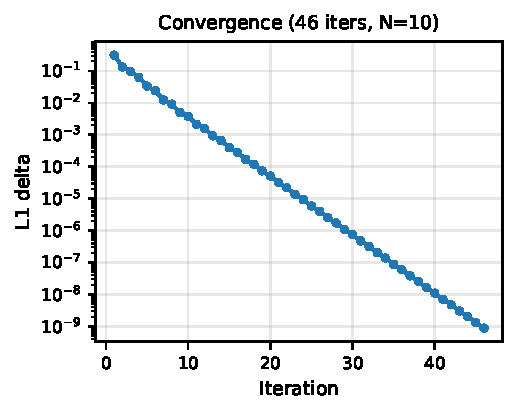
\includegraphics[width=\columnwidth]{figures/convergence.pdf}
\caption{$L_1$ delta per iteration for the reference engine. The error decreases
monotonically and crosses $\varepsilon=10^{-3}$ at iteration 13.}
\label{fig:convergence}
\end{figure}

\begin{figure}[t]
\centering
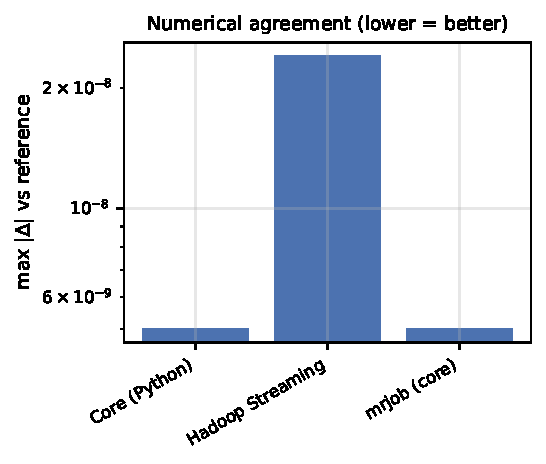
\includegraphics[width=\columnwidth]{figures/accuracy.pdf}
\caption{Maximum per-node disagreement with the reference engine (log scale,
lower is better). Differences sit at the eight-decimal output-precision floor.}
\label{fig:accuracy}
\end{figure}

\subsection{Single-node performance and scaling}
Table~\ref{tab:perf} and Figures~\ref{fig:runtime}--\ref{fig:memory} report
wall-clock time and peak memory for the three frameworks that run on a single
node without a cluster: the pure-Python engine, mrjob's local MapReduce, and the
Hadoop Streaming local pipeline. The in-memory engine is fastest at every size;
mrjob adds a modest constant overhead from its runner; and Hadoop Streaming is
the slowest by an order of magnitude because it spawns operating-system
processes and re-serializes the entire state through the
\texttt{map$\,|\,$sort$\,|\,$reduce} pipeline on every iteration. Conversely,
Streaming's peak memory is the lowest, since it streams records rather than
holding the graph in a single address space---a concrete illustration of the
classic time--memory trade-off between in-memory and streaming execution.

\begin{table}[t]
\centering
\caption{Single-node wall-clock time (s) and peak memory (MB), 30 iterations,
Barab\'asi--Albert graphs. Measured in the CI container.}
\label{tab:perf}
\begin{tabular}{@{}lrrr@{}}
\toprule
 & $N{=}10^3$ & $N{=}5\!\times\!10^3$ & $N{=}10^4$ \\
\midrule
Core (Python)    & 0.12\,s / 13.4 & 0.67\,s / 18.4 & 0.87\,s / 24.6 \\
mrjob (core)     & 0.21\,s / 24.5 & 1.05\,s / 29.2 & 1.14\,s / 35.5 \\
Hadoop Streaming & 1.57\,s / \phantom{0}9.6 & 3.41\,s / 11.6 & 7.56\,s / 13.9 \\
\bottomrule
\end{tabular}
\end{table}

\begin{figure}[t]
\centering
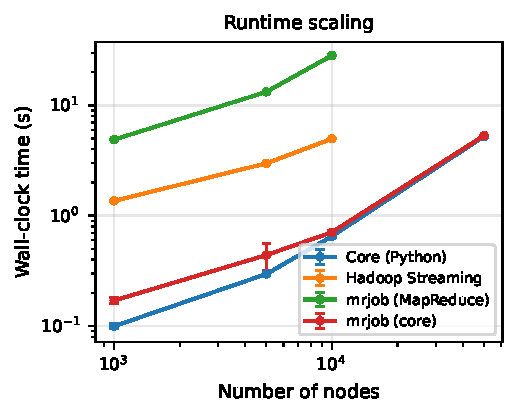
\includegraphics[width=\columnwidth]{figures/runtime_scaling.pdf}
\caption{Wall-clock time vs.\ graph size (log--log). The in-memory engine and
mrjob scale near-linearly in $|E|$; the Streaming pipeline carries a large
per-iteration constant.}
\label{fig:runtime}
\end{figure}

\begin{figure}[t]
\centering
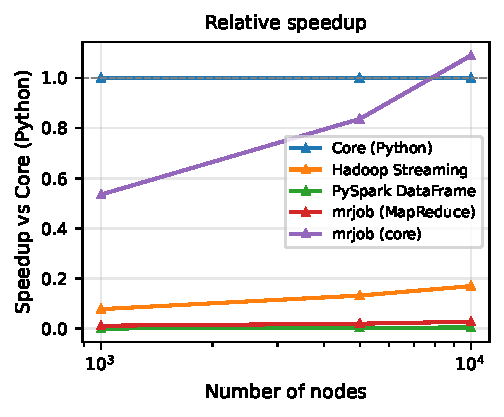
\includegraphics[width=\columnwidth]{figures/speedup.pdf}
\caption{Speedup relative to the pure-Python baseline. Values below~1 indicate
slower execution; the framework overheads dominate at these single-node sizes.}
\label{fig:speedup}
\end{figure}

\begin{figure}[t]
\centering
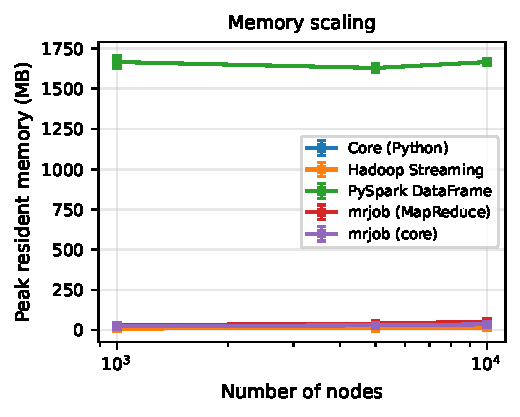
\includegraphics[width=\columnwidth]{figures/memory_scaling.pdf}
\caption{Peak resident memory vs.\ graph size. The streaming pipeline trades
runtime for the smallest memory footprint.}
\label{fig:memory}
\end{figure}

These single-node results quantify framework \emph{overhead}: at $10^4$ nodes the
graph fits comfortably in memory, so the distributed machinery only adds cost.
The regime in which Spark and Hadoop repay their overhead---graphs whose edge
sets exceed single-node memory---lies beyond what a single container can
measure; we discuss this boundary in Section~\ref{sec:discussion} and treat its
empirical characterization as future work (Section~\ref{sec:limits}).

\section{Discussion}
\label{sec:discussion}
\textbf{Where overhead comes from.} Every implementation performs $O(|E|)$ work
per iteration, so asymptotically they are equivalent; the measured differences
are constants. The pure-Python engine pays only interpreter overhead. mrjob's
inline runner adds protocol (de)serialization between map and reduce. Hadoop
Streaming additionally pays process-creation and full-state re-serialization each
iteration, which explains its order-of-magnitude slowdown and its
super-linear-looking growth at small sizes. In-memory Spark is designed to
eliminate exactly this per-iteration I/O, but only once the data is large enough
that the fixed cost of standing up executors is amortized.

\textbf{Iterative lineage must be truncated.} A subtle but critical finding
concerns Spark's lazy evaluation: chaining a self-join per iteration grows the
logical/physical query plan without bound, and the driver eventually exhausts
its heap while merely \emph{rendering} the plan. Caching is insufficient because
it does not cut lineage. We resolved this by checkpointing each iteration's rank
vector (\texttt{localCheckpoint}), which materializes the result and truncates
the plan. This is a general lesson for any iterative algorithm expressed in
Spark, not specific to PageRank.

\textbf{Engineering pitfalls across frameworks.} Porting one algorithm to many
runtimes surfaced several environment-specific defects that never manifest in the
pure-Python reference: (i) Spark resolved relative input paths against the
cluster's default filesystem (HDFS) rather than the local disk, fixed by
emitting explicit \texttt{file://} URIs for scheme-less paths; (ii) the
DataFrame convergence check used an aliased self-join that is fragile to analyzer
ambiguity, replaced by explicit column renaming; (iii) \texttt{RDD.localCheckpoint()}
returns \texttt{None} (it marks the RDD in place), unlike its DataFrame
counterpart, so re-binding the variable silently produced a null dataset; and
(iv) \texttt{mrjob} depends on \texttt{distutils}, removed in Python~3.12, so the
test harness must detect and skip it on newer interpreters. None of these are
algorithmic errors, yet each would silently corrupt results or crash a job in
production; cataloguing them is, we argue, as valuable as the performance
numbers.

\textbf{Choosing a framework.} For graphs that fit in memory, a plain in-memory
implementation is simplest and fastest; the distributed frameworks are justified
by data volume, fault tolerance, and integration with an existing cluster, not by
single-node speed. Among the distributed options, the relational DataFrame API is
the most concise and benefits from Catalyst, the RDD API offers the most explicit
control, and the MapReduce/Streaming/Pig variants are most appropriate where a
Hadoop stack is already the operational standard.

\section{Limitations and Future Work}
\label{sec:limits}
Our performance comparison is single-node and therefore measures framework
overhead rather than distributed scalability; the PySpark, Java, and Pig engines
are validated for correctness but their cluster-scale behaviour is not yet
measured here. The benchmark harness already supports these runtimes, so the
natural next step is a multi-node study on graphs with $10^6$--$10^7$ edges
(e.g.\ SNAP datasets~\cite{leskovec2014}), reporting strong- and weak-scaling for
Spark. Further work includes redistributing dangling mass in the single-pass
JVM/Streaming jobs via a global aggregation step, adding Topic-Sensitive
PageRank, and comparing against vertex-centric engines such as
GraphX~\cite{gonzalez2014}.

\section{Conclusion}
\label{sec:conclusion}
We presented a single-codebase comparative study of PageRank across the Hadoop
ecosystem, anchored by a dependency-free reference engine and an independent
NetworkX oracle. Six implementations were shown to be numerically equivalent up
to output precision, after which a reproducible single-node benchmark quantified
their overhead: an in-memory engine dominates at sizes that fit in memory, while
distributed frameworks add cost that is repaid only at scale. Beyond the
measurements, the study contributes a concrete catalogue of cross-framework
engineering pitfalls and a configuration-driven harness that extends directly to
cluster-scale evaluation. We hope both the methodology---validate first, then
compare---and the reproducible artifacts are useful to practitioners selecting an
execution model for iterative graph computation.

\begin{thebibliography}{99}
\bibitem{brin1998} S.~Brin and L.~Page, ``The anatomy of a large-scale
hypertextual web search engine,'' \emph{Computer Networks and ISDN Systems},
vol.~30, no.~1--7, pp.~107--117, 1998.

\bibitem{page1999} L.~Page, S.~Brin, R.~Motwani, and T.~Winograd, ``The PageRank
citation ranking: Bringing order to the web,'' Stanford InfoLab, Technical
Report, 1999.

\bibitem{dean2008} J.~Dean and S.~Ghemawat, ``MapReduce: Simplified data
processing on large clusters,'' \emph{Communications of the ACM}, vol.~51,
no.~1, pp.~107--113, 2008.

\bibitem{zaharia2012} M.~Zaharia \emph{et al.}, ``Resilient distributed datasets:
A fault-tolerant abstraction for in-memory cluster computing,'' in \emph{Proc.
USENIX NSDI}, 2012.

\bibitem{armbrust2015} M.~Armbrust \emph{et al.}, ``Spark SQL: Relational data
processing in Spark,'' in \emph{Proc. ACM SIGMOD}, 2015, pp.~1383--1394.

\bibitem{olston2008} C.~Olston, B.~Reed, U.~Srivastava, R.~Kumar, and
A.~Tomkins, ``Pig Latin: A not-so-foreign language for data processing,'' in
\emph{Proc. ACM SIGMOD}, 2008, pp.~1099--1110.

\bibitem{malewicz2010} G.~Malewicz \emph{et al.}, ``Pregel: A system for
large-scale graph processing,'' in \emph{Proc. ACM SIGMOD}, 2010,
pp.~135--146.

\bibitem{gonzalez2014} J.~E.~Gonzalez \emph{et al.}, ``GraphX: Graph processing
in a distributed dataflow framework,'' in \emph{Proc. USENIX OSDI}, 2014,
pp.~599--613.

\bibitem{barabasi1999} A.-L.~Barab\'asi and R.~Albert, ``Emergence of scaling in
random networks,'' \emph{Science}, vol.~286, no.~5439, pp.~509--512, 1999.

\bibitem{hagberg2008} A.~A.~Hagberg, D.~A.~Schult, and P.~J.~Swart, ``Exploring
network structure, dynamics, and function using NetworkX,'' in \emph{Proc. 7th
Python in Science Conf. (SciPy)}, 2008, pp.~11--15.

\bibitem{leskovec2014} J.~Leskovec and A.~Krevl, ``SNAP Datasets: Stanford large
network dataset collection,'' \url{http://snap.stanford.edu/data}, 2014.

\bibitem{lin2010} J.~Lin and C.~Dyer, \emph{Data-Intensive Text Processing with
MapReduce}. Morgan \& Claypool, 2010.
\end{thebibliography}
